\clearpage
\section{浴室墙砖上的三角形}
浴室的墙砖和柜门都是平面。照在同一块柜门上的光可以逐渐变弱，但不该沿着三角形的对角线突然变暗。换成光栅绘制第一层表面后，柜门上出现一块块尖角，大理石的白纹也消失了。这个场景恰好可以把两种问题分开看。材质的底色图应当保留石纹；记录表面朝向的法线图里，同一块平门应有一致的颜色。

\begin{figure}[H]\centering
\begin{minipage}[t]{.48\linewidth}\centering
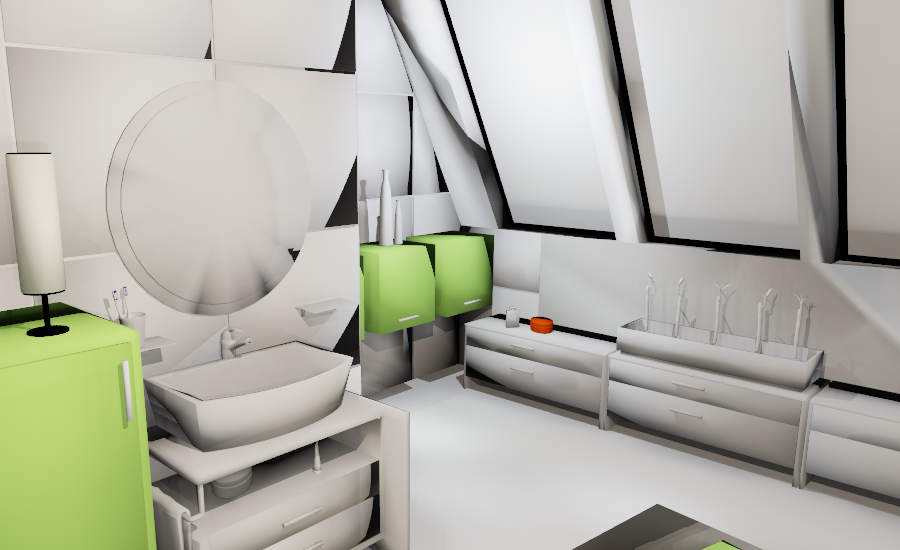
\includegraphics[width=\linewidth]{../../../output/validation/bathroom/before.png}\\
{\small 修正前}
\end{minipage}\hfill
\begin{minipage}[t]{.48\linewidth}\centering
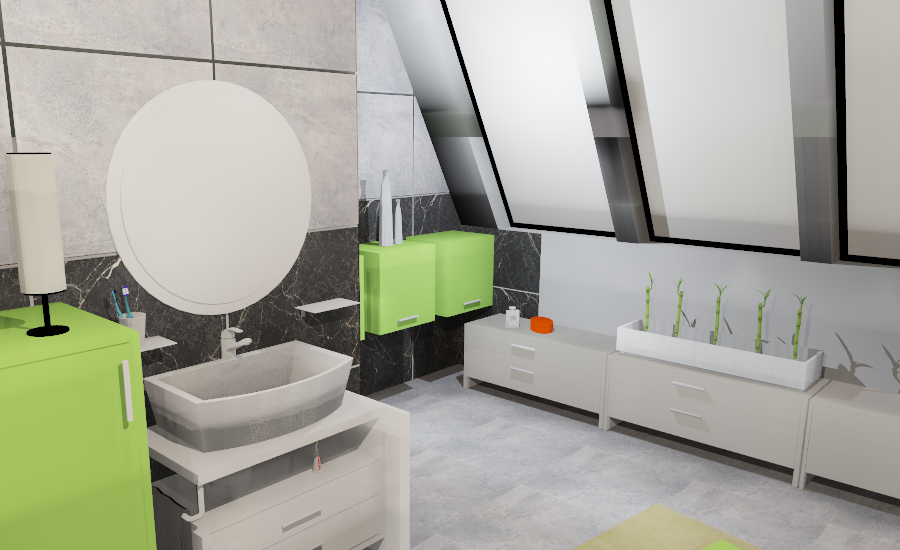
\includegraphics[width=\linewidth]{../../../output/validation/bathroom/after.png}\\
{\small 修正后}
\end{minipage}
\caption{同一浴室与相机，两次正式 Vulkan 编辑器运行的第 12 帧。先看圆镜两旁的墙砖，再看右边矮柜。两图从 $1391\times892$ 像素的显示输出裁取同一区域。模型为 cenobi 创作的 Bathroom，由 NVIDIA RTXGI 收录，CC BY 3.0。}
\end{figure}

模型用 GLB 保存，九张图片都打包在模型内部。导入器 Assimp 给这种图片取 \verb|*0|、\verb|*1| 等名字，星号后的数字是图片在数组中的序号。旧的 \path{Model.cpp} 遇到这种名字便跳过，场景退回到材质常量色。照片式的大理石纹自然也没有进入底色图。

\begin{Code}
// 原来的贴图路径处理。GLB 把图片存在文件内部。
if (texPath.data[0] == '*')
    return "";
\end{Code}

现在 \verb|Model::LoadMaterialTexture| 用 \verb|FindModelImage| 读出 GLB 内嵌的 RGBA 像素。浴室 85 个几何部件都缺少 \verb|NORMAL|。glTF 规定此时每个三角形应取自己所在平面的法线。早期对照同时修了贴图导入，并把平滑法线改为 \verb|aiProcess_GenNormals|。墙砖的花纹已回来，两张组合光照图本身不能独立证明法线的生成过程正确。

后来用一块正对镜头的色板单测法线：几何在 XY 平面上，正确朝向应是 $+Z$。在 RenderDoc 第 27 个事件却读到 $+Y$。查到项目编译 Assimp 时关闭了平面法线生成器，即使调用者给出正确标志，过程也不会运行。根目录的 \path{premake5.lua} 现已启用这个生成器，重新编译后，同一像素读到 $+Z$。\href{run:../profiling/material-channels/README.md}{正式色板的法线图与逐像素记录}

从仓库根目录运行 \path{python tests/fetch_rtxgi_bathroom.py}，再双击 \path{RTXGI-Bathroom.redflag} 即可复看。同一门内机位也留有新版点光源、材质与四轮探针的截图。\href{run:../profiling/point-materials/bathroom-pbr.png}{浴室现版实拍}

\note{\href{run:../../Redflag/src/Redflag/Renderer/Model.cpp}{Model.cpp · Load 与 LoadMaterialTexture}\quad
\href{https://registry.khronos.org/glTF/specs/2.0/glTF-2.0.html\#meshes}{Khronos · 网格法线}\quad
\href{run:../validation/bathroom/README.md}{两次输出与来源}}

\clearpage
\section{首次绘制玻璃时的模型上传}
打开玻璃展台时，编辑器已经能画自己的内建立方体，玻璃用的模型却要到第一次访问才会加载。这个先后顺序暴露了一个启动错误。2026 年 11 月 22 日的 Debug x64 运行打开场景、记录了平面材质，随后进程退出；Windows 报告驱动模块 \verb|nvoglv64.dll| 访问冲突。只有已经上传完全部网格的离屏测试此前一直可以通过。

模型的顶点和贴图要先从暂存区域传到显存，然后 GPU 才能绘制。\verb|VulkanDraw::DrawSurfaces| 原先借用上传用的命令池来录制整遍几何。第一次遇到还没上传的模型时，创建网格和贴图也调用 \verb|ImmediateSubmit|。它的第一步恰好就是把上传命令池重置。此时外层还在录制刚才的墙面，重置会使这份尚未提交的命令失效。下面的伪代码压缩了这次出错的调用次序。

\begin{Code}
recordSurfaces(uploadPool);     // 墙面的命令仍在录制
    uploadTexture(uploadPool);  // 创建贴图时重置了同一个池
    drawGlass();                // 外层试图继续录制
\end{Code}

修正后，\verb|VulkanContext| 给录制表面与上传资源分别留了一套命令池、命令缓冲和完成信号。两个池仍使用同一条图形队列。模型上传完成后，绘制可以继续写自己的命令；首次收集照明所用几何时，也会加载场景引用的模型，避免第一帧漏掉它的遮挡。这里仍然会等待上传和这次离屏工作完成，更细粒度的帧内调度需要独立计时验证。

为了直接覆盖这次的先后顺序，\verb|tests/RHITests.cpp| 的 \verb|CheckLightingSurfaces| 先录一笔远处网格，在回调中上传一张 $1\times1$ 的贴图，然后继续录近处网格。分别使用透视和正交投影，读回两层重合处，必须得到远处网格的绿色和实体号 42，背景仍为空。在仓库根目录运行 \path{tests/run_rhi_tests.cmd} 可以复测。正式编辑器也重新打开了展台，两种折射率均记录到第 12 帧，透明阶段有两次实际绘制，回放未出现验证消息。

\note{\href{run:../../Redflag/src/Platform/Vulkan/VulkanContext.cpp}{VulkanContext.cpp · ImmediateSubmit}\quad
\href{run:../../Redflag/src/Platform/Vulkan/VulkanDraw.cpp}{VulkanDraw.cpp · DrawSurfaces}\quad
\href{run:../scenes/glass-studio/capture.json}{两次运行的 RenderDoc 记录}}
